\chapter{The Names of Spices}
\label{ch:names}

% \setlength\intextsep{0pt}

% Empirical Chapters
% Discuss and present your findings in a factual way.
% What are the results of your investigations?
% How do the findings relate to previous studies?
% Was there anything surprising or that didn’t work out as planned?
% Are there any themes or categories that emerge from the data?

\lettrine[lines=\iniciale]{\textcolor{\accentcolor}{N}}{ow} that the detailed introduction of the spices is complete, let us examine these spice names comparatively as three sets representing the nomenclature in English, Arabic, and Chinese. This chapter constitutes the analysis and findings part of the thesis, and will thematically introduce certain aspects of the terminology of the spice domain, guiding the reader from a general overview towards more nuanced probes that can be derived from the results. The aim of this chapter is to showcase the many ways we can interpret, analyze, and visualize the data.

% I will cover multiple investigations, ranging from the percentage of loanwords, to the use of color-words in the names.

\section{Overview: Figures and Statistics}

\begin{wrapfigure}{R}{0.33\textwidth}
  \vspace{-\baselineskip}
  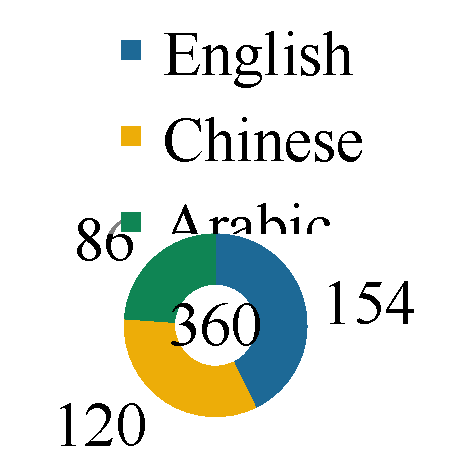
\includegraphics[width=0.33\textwidth]{imgs/plots/languages_pie.pdf}
  \caption{The distribution of spice names across the three languages.}
  \label{fig:languages_pie}
\end{wrapfigure}

As a result of the data collection set forth in \cref{ch:data}, the database now contains 369 spice names. Of these, 159 are in English, 87 are in Arabic, and 123 are in Chinese; \cref{fig:languages_pie} shows this distribution.
The total number is the accumulation of the lengthy process of carefully compiling the nomenclature for the set of spices as defined at the beginning of the thesis, which consists of 24 different spices. The data collection methods were detailed in \cref{sec:data_collection}. 

On average, a spice has 14 names, where the max is 44 (chile), the min is 4 (fenugreek and mace). \Cref{fig:ids_top_and_bottom_ann} show the top ten and the bottom ten spices that have the most and least number of names including all three languages. This measurement might raise some eyebrows, but in fact it is a very good indicator of which spices are more complex in their nomenclature, and therefore which are the most ``problematic'' to untangle. As we can see, spices that boast with many names include the chili pepper, Sichuan pepper, cassia, false cardamoms, and allspice. These are---not incidentally---the very items that I have dedicated substantially more pages to than some of the other spices, due to issues about their identity or the complexity and richness of their nomenclature. This seems to go hand in hand with matters of biodiversity: chile has countless varieties that have spread to faraway corners of the earth, and now it is a hobby in its own right to cultivate, breed, and crossbreed hot chili pepper cultivars. As we saw, Sichuan peppers species are used across vast regions, and it can cause headache to pin them down exactly, their ``boundaries'' are not that well defined, and it also needed some explanation to isolate the various sources of cassia types.

On the other hand, spices with the lowest number of names are presumably the most straightforward items, take for example cloves, or vanilla. But What makes a spice ``straightforward'', or in other words, simple? In my opinion, it is their uniqueness and recognizability. Indeed, if we reflect on our investigation on vanilla in the last section of the previous chapter, we have already established that it is a rather special item: there is no other spice that is made from the fruits of an orchid---it is unique. Or, if we think of cloves, they are unmistakable in their shape and in many language they are known by their shape (see \ref{ety:clove}). These two items are also very well circumscribed in terms of their geographic origins. Although now cultivated in multiple tropical regions, vanilla is known to be from the jungles of Central America and Brazil, there is no doubt about its origins. The native habitat of cloves is even more narrow, as it is only indigenous only to North Maluku and the ``spice islands'' of Makian, Ternate, and Tidore. We see nutmeg and mace as well among the bottom five items with the least amount of names, and we should notice that nutmeg and its mace are also from this region, they were exclusively found on the Banda islands of Maluku, and nowhere else until the second half of the \nth{18} century. Now, it makes a bit more sense to look at these same charts deconstructed by language, this can be seen on \cref{fig:ids_trio}. The most conspicuous feature of these pie charts is that chili has the most names, across every language.

% \begin{figure}[!ht]
% 	\centering
% 	\subfloat[Top 10]{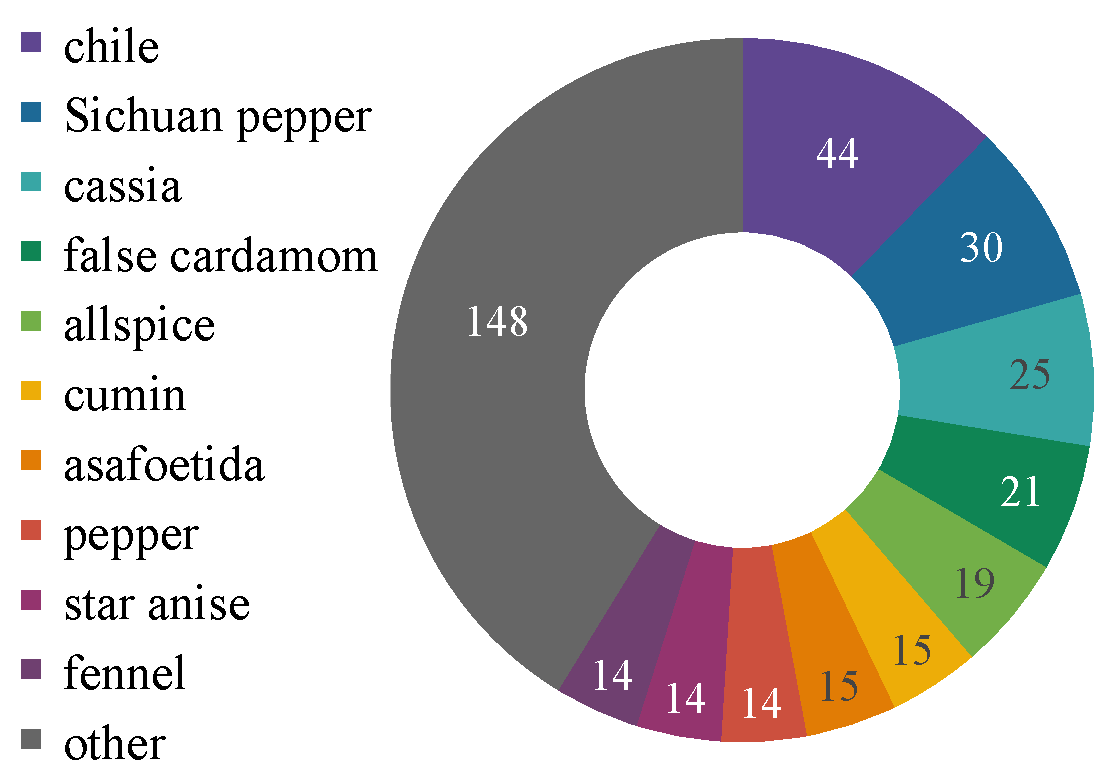
\includegraphics[width=0.5\linewidth]{imgs/plots/ids_top_pie.pdf}}
% 	\hfill
% 	\subfloat[Bottom 10]{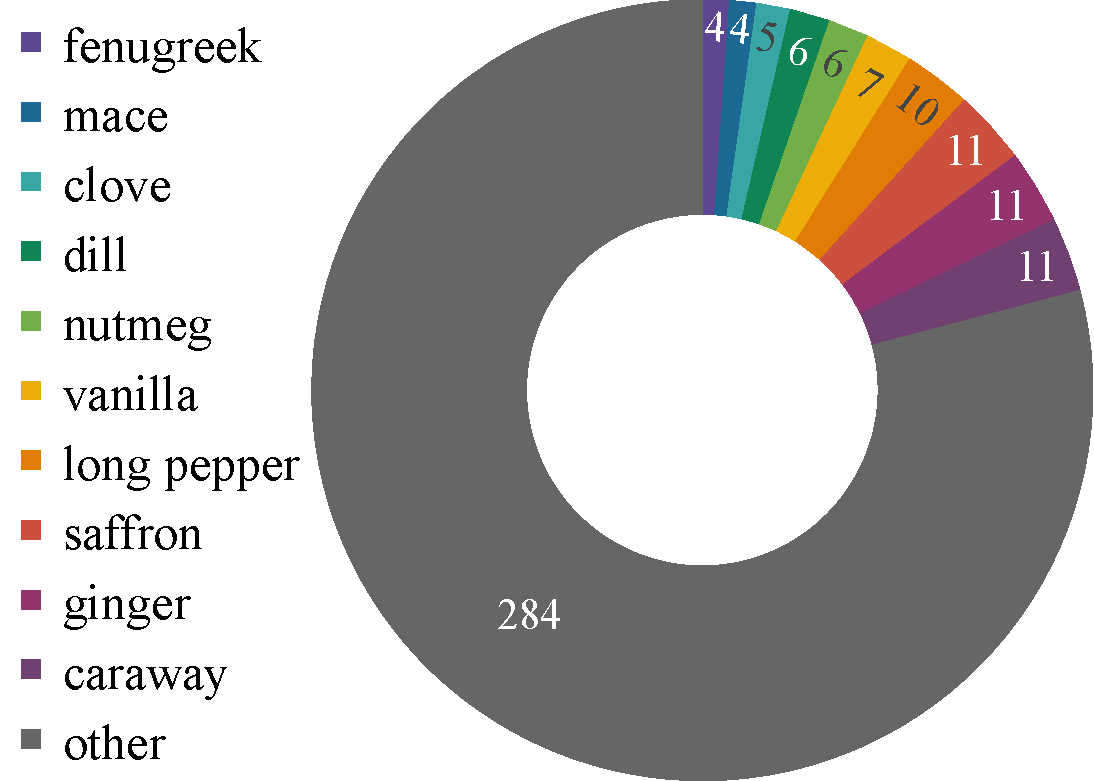
\includegraphics[width=0.5\linewidth]{imgs/plots/ids_bottom_pie.pdf}}
% 	\caption{}
% 	\label{fig:ids_top_and_bottom}
% \end{figure}

\begin{figure}[!ht]
	\centering
	\subfloat[]{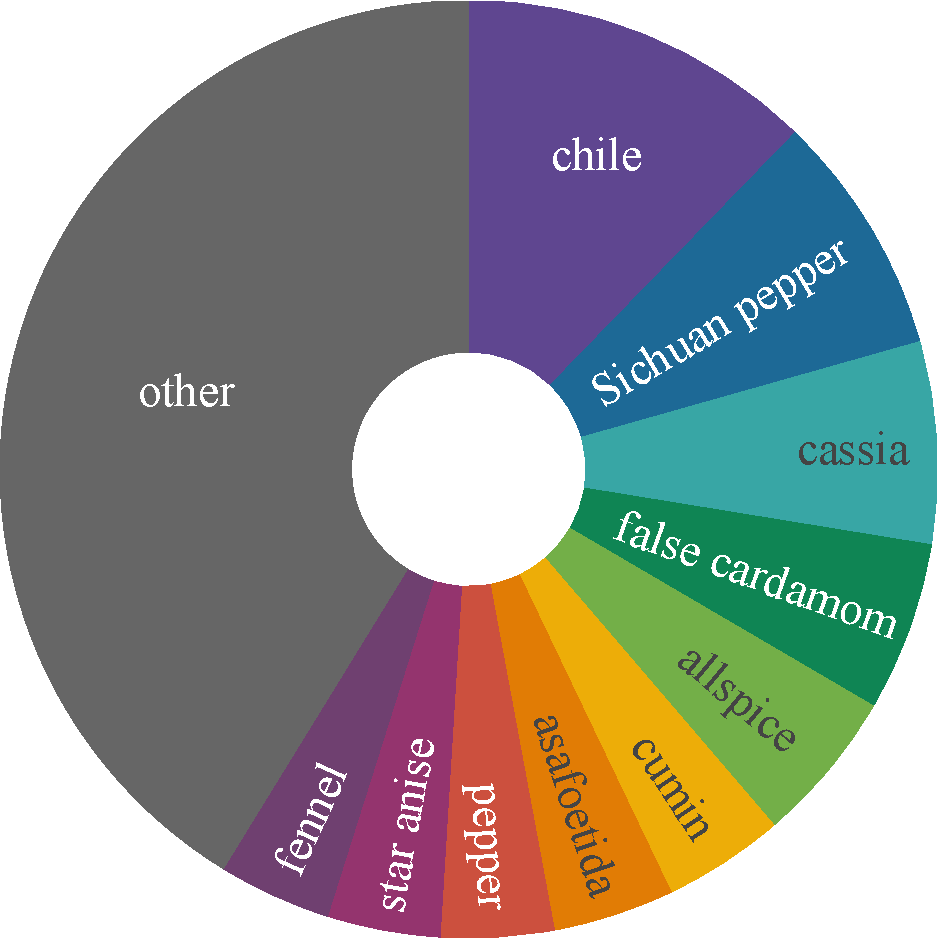
\includegraphics[width=0.5\linewidth]{imgs/plots/ids_top_pie_ann.pdf}}
	\hfill
	\subfloat[]{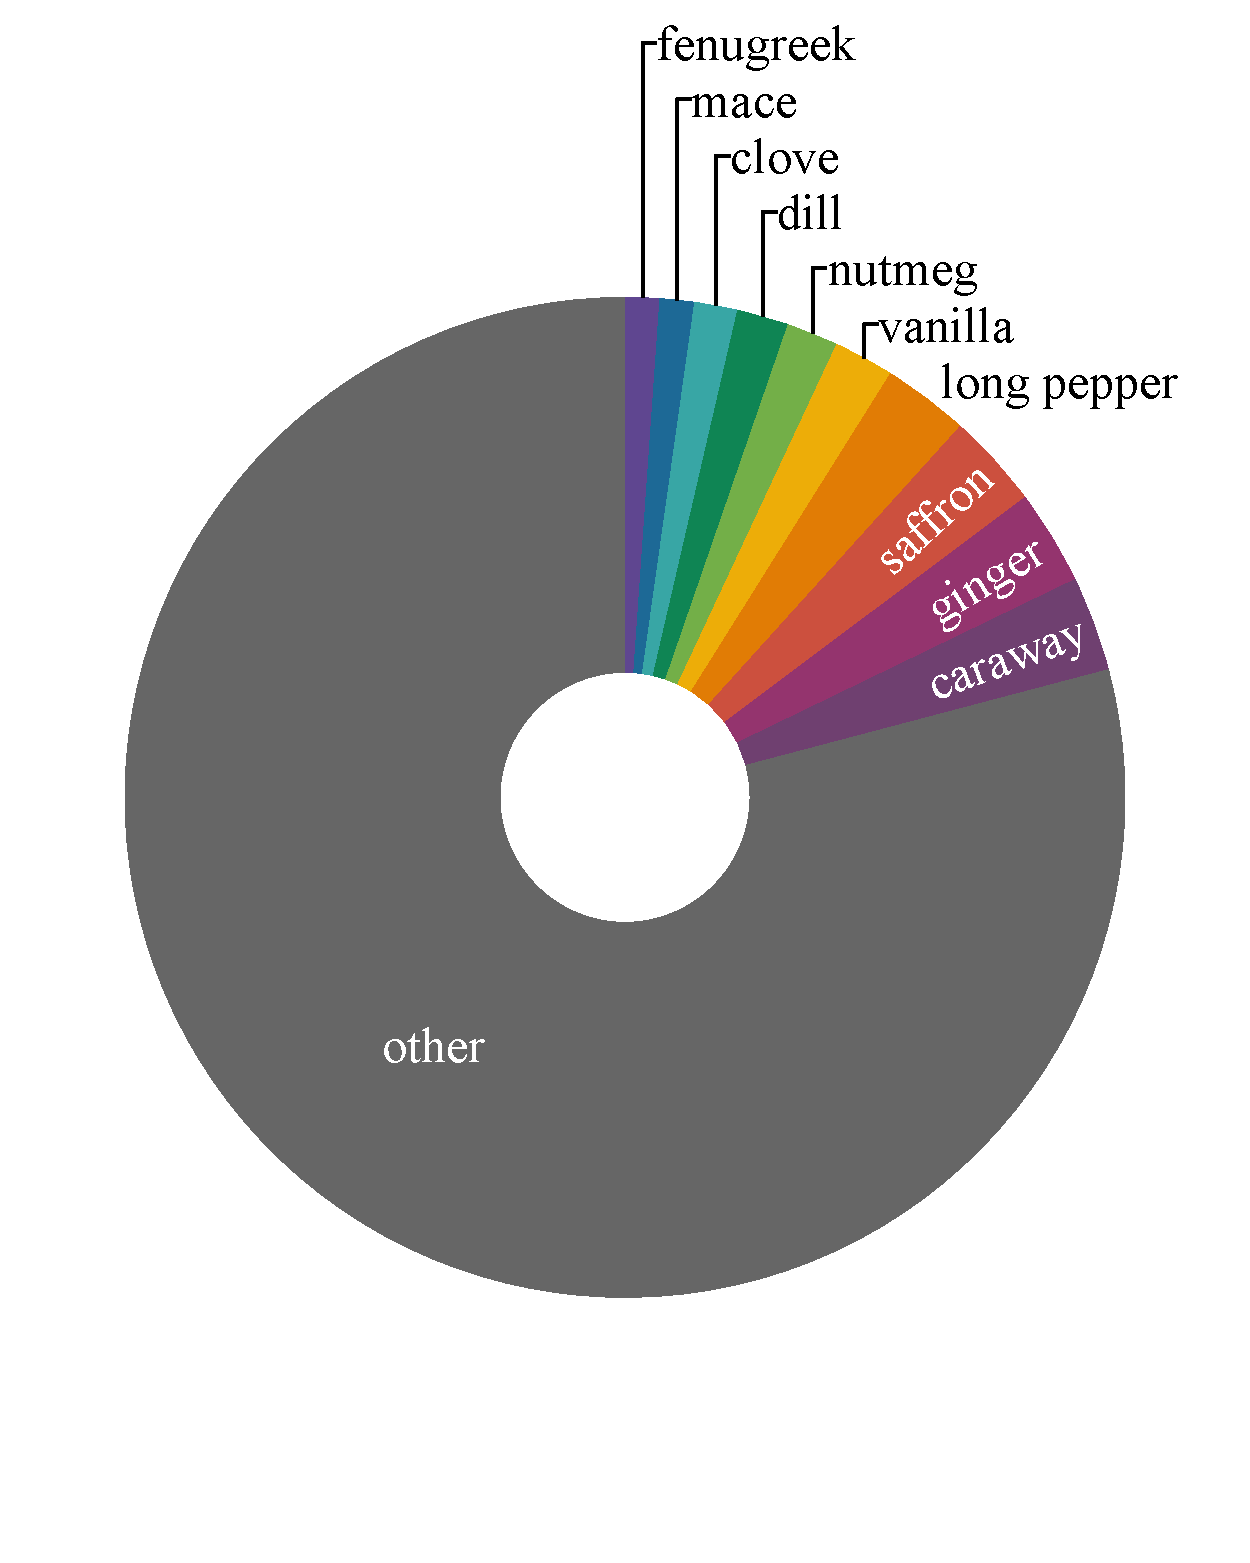
\includegraphics[width=0.5\linewidth]{imgs/plots/ids_bottom_pie_ann.pdf}}
	\caption[Top and bottom spices by number of names.]{Top 10 spices with the most number of names (a), and bottom 10 spices with the least number of names (b).}
	\label{fig:ids_top_and_bottom_ann}
\end{figure}

\begin{figure}[!ht]
	\centering
	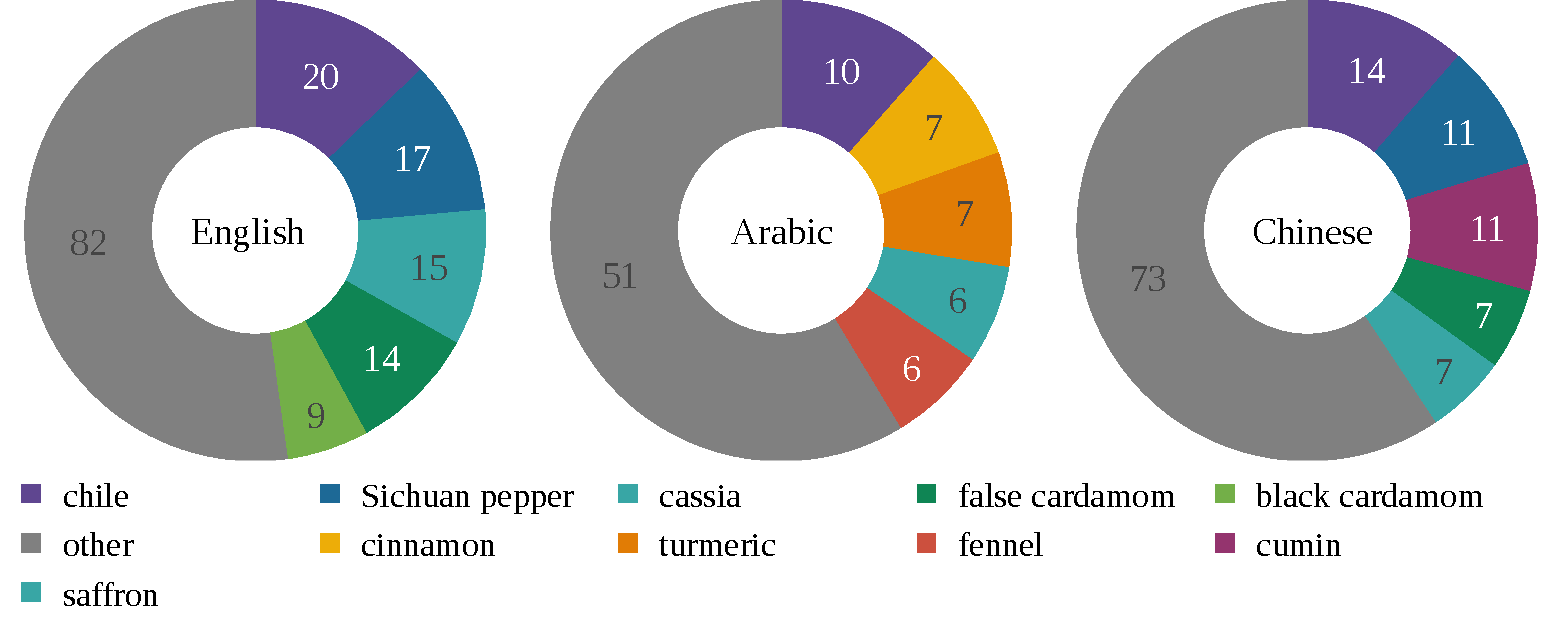
\includegraphics[width=\linewidth]{imgs/plots/ids_trio.pdf}
	\caption[Top spices by number of names, broken down by language.]{Top 5 spices with the most number of names, broken down by language.}
	\label{fig:ids_trio}
\end{figure}



% Trivially, the more similar some spices are, the more confusing their nomenclature will get. The best example for this are the spices from the umbel family: cumin, caraway, anise, fennel, dill, and so on; little seed-like fruits that grow from the Mediterranean to Central Asia. The fascinating connections are most visible when examining them in multiple languages. % EXAMPLES 

% According to the \gls{WN}, there are four senses to the noun \textit{pepper}. Two refers to \textit{Capsicums}, and two to ``true peppers''. Pepper\#1 in the plant lexical file, with synonyms of common pepper\#1, black pepper\#1, white pepper\#1, Madagascar pepper\#1, and Piper nigrum\#1 is defined as ``climber having dark red berries (peppercorns) when fully ripe; southern India and Sri Lanka; naturalized in northern Burma and Assam''. Its hyponym is pepper\#3, synonym of peppercorn\#1, with the definition ``pungent seasoning from the berry of the common pepper plant of East India; use whole or ground'', now we are in the food lexical file. This latter, has two hyponyms on its own: black pepper\#2 (``pepper that is ground from whole peppercorns with husks on'') and white pepper\#2 (``pepper ground from husked peppercorns'')

% How to accommodate for the confusion in the past, semantic changes kurkum, saffron? They appear twice in both relevant categories! 

\section{The Analysis of Spice Nomenclature}

This chapter will present the analysis on these spice names, and try to answer the main question: How do people name spices, specifically, new spices that they came into contact with? Immediately, we can think of two ways: languages either borrow, or conceive a name. But how does this naming process work exactly? What are the underlying mechanisms and critical factors that influence the naming, and how does the nomenclature reflect the contact situation? How does borrowing work, and how languages invent new names for novel materials and substances? In an attempt to give answers to these questions, I will take a bottom-up approach and look at examples from the data I collected to arrive to some conclusions.

\subsection{Terminology}
During the analysis, I will take into account the term's (a) analyzability, their (b) borrowed status, and inspect the ways spice terms are generated using (c) prototype words and distinguishing words.

\subsubsection{Analizability}

Analyzability of words is an idea from the \nth{20}-century philological movement and method \textit{Wörter und Sachen} (words and things in German), which had a big influence on linguistics and ethnography. Outlined by Hugo Schuchardt and based on the titular journal \textit{} started by Indo-Europeanist Rudolf Meringer in 1909, it proposed the close study of the etymology of words together with the artifacts/concepts \autocite{ortutay_magyar_1977}. 

% A Wörter und Sachen ('Szavak és dolgok') a Hugo Schuchardt által kidolgozott, a nyelvészetre és a néprajzra mély hatással lévő módszer, a tárgyak és szavak kölcsönös kutatásának elve, eredetileg R. Meringer indoeurópai nyelvész 1909-ben indított folyóiratának címe.
% A módszer lényege: a szavak vándorlásában (kölcsönszavak) nem elegendő pusztán csak a megfelelő korban működő és ható hangtörvényekre és esetleg a szó jelentésére támaszkodni, hanem a nyelvi tények tanulmányozásán kívül vizsgálni kell a szavaktól jelölt dolgokat és tárgyakat. Természetesen itt számolni kell még művelődéstörténeti tényezőkkel is.
% A módszert Ferdinand Blumentritt, valamint Jankó János és Bátky Zsigmond is sikeresen használta fel. 

% Wörter und Sachen

% R. Meringer indoeurópai nyelvész 1909-ben megindított folyóirata, amelyben ő és munkatársai azt a módszert képviselték, hogy a szavak jelentésfejlődésének és eredetének kutatásánál a néprajz – a tárgyak, jelenségek, intézmények, szokások vizsgálatánál pedig a nyelvészet (elsősorban a szótörténet, etimológia) eredményeit figyelembe kell venni. A néprajzi tárgykutatás jelentőségét emelte ki Meringer akkor, amikor 1906-ban azt írta, hogy „Ohne Sachwissenschaft keine Sprachwissenschaft mehr!” (’Tárgyi tudomány nélkül nincs többé nyelvtudomány’). A Wörter und Sachen a tárgyak és szavak kölcsönös kutatásának elvét Jankó János és Bátky Zsigmond eredetmagyarázataiknál (halászat, építkezés) körültekintően alkalkazták. A Wörter und Sachen módszerével tanulságos eredményeket ért el újabban Balassa Iván: A magyar kukorica (Bp., 1960). A Wörter und Sachen módszere különösen fejlett a finn (U. T. Sirelius, K. Vilkuna, N. Valonen, T. Vuorela) és az észt (F. Linnus, G. Ränk, A. Viires) etnográfusok körében. A Wörter und Sachen módszerével dolgozta fel F. Krüger a Pireneusok néprajzát. – Irod. Meringer, R.: Indogermanische Forschungen (Wien, 1906).

``Ohne Sachwissenschaft keine Sprachwissenschaft mehr!'' There is no linguistics anymore without the study of material culture!

Basically, the more opaque a name is in terms of morphological analysis, the longer it is assumed to be present in the language. A basic example would be \textit{York} (monomorphemic) vs. \textit{New York} (analysable), which provides a potential chronology for the concepts the words signify. This approach was incorporated into historical linguistic research and philology, often studied in parallel with findings in archeology. SOURCE??

\textcite[12]{haspelmath_loanwords_2009} also used the term ``analyzability'' in the creation of their loanword database (\gls{WOLD}) as a first step to assess a word's loanword status, although --- to the grief of --- in a purely linguistic way. 

% Contributors were asked to indicate whether the word was (1) unanalyzable (if the form could not be analyzed into two or more constituents); (2) semi-analyzable (if a constituent structure could be identified, but not all constituents had meanings, such as a “cranberry morph”; or if the word was analyzable to linguists but not to lay speakers); (3) analyzable derived; (4) analyzable compound; (5) analyzable phrasal. For analyzable items, contributors were asked to give a morpheme-bymorpheme gloss, i.e. a hyphenation and a gloss in square brackets. For example, for Kanuri shàdàmá ‘witness ’, the field contains the following: “shàdà-má [testimonyowner.of]”. For abbreviations of grammatical categories, contributors were referred to the Leipzig Glossing Rules.

If the word is morphosyntactically complex, ``it was almost certain that it was created by speakers of the language rather than borrowed from some other language'' --- we can read. The authors also state that these are not considered loanwords, even when they contained borrowed elements. 

\subsubsection{Borrowed Word or Native Invention}

Closely related to analyzability, is the question if a term is borrowed or not.

% 5.3. Borrowed Most importantly, of course, contributors were asked to indicate whether, to the best of their knowledge, the word was a loanword, i.e. had been borrowed from another language at some point in the language’s history. Protolanguages were also considered stages of the same language, so that a word borrowed into Proto-Uralic, for example, would count as a loanword in Saami. Five degrees of certainty were distinguished

% I. The Loanword Typology project and the World Loanword Database 13 0. No evidence for borrowing 1. Very little evidence for borrowing 2. Perhaps borrowed 3. Probably borrowed 4. Clearly borrowed A value such as “Clearly not borrowed” or “Clearly inherited” was not used, because any word could have been borrowed at some prehistoric time, so we can never be sure that a word is not an old loanword. And even loanwords can be inherited, e.g. a word borrowed into Proto-Uralic can be inherited by Saami. We define a loanword as a lexeme that has been transferred from one lect into another and is used as a word (rather than as an affix, for example) in the recipient language. Words from a substrate language, too, were considered to be loanwords for the purposes of the LWT project, so we include both adopted and imposed words (see chapter II, §2, §7.4). Lexemes transferred from one regional dialect to another and between an acrolect and a basilect were also treated as loanwords in principle, although in practice they play a minor role. Excluded from the class of loanwords are neologisms (= productively created lexemes) which consist partly or entirely of foreign material, because they are created in the recipient language, and not transferred from a donor language (cf. §5.5.4; but see “calqued” in §5.5.3). 5.4. Age For each word, contributors gave the earliest time at which it was attested or could be reconstructed in the language. For loanwords, this meant the time when the word was borrowed. For nonloanwords, it meant the time of earliest attestation or reconstruction. Dates could be indicated by years (or centuries) or by period name, e.g. “Middle High German”, or “Tang dynasty”, in which case contributors were asked to provide approximate dates for the periods, e.g. 1050–1350 for “Middle High German”, 618–907 for “Tang Dynasty”, and 5000–3000 BCE for “ProtoIndo-European”. Knowing the age of a word is important in this context for several reasons. For nonloanwords which have only existed in the language for a relatively short period, it is not possible to draw conclusions regarding borrowability: they may be replaced by a loanword given sufficient time. On the other hand, a word that has been present in a language for a thousand years without being replaced by a loanword provides good evidence that its meaning is less borrowable. For older loanwords, tracing their origin can be more rewarding since we are less likely to know the history of their borrowing situation compared to newer loanwords. Studying old loanwords can thus help fill important gaps in historical and archeological knowledge. Finally, in a diverse sample such as ours, the history of some languages is relatively well documented for thousands of years, while others have only been re

% 14 Martin Haspelmath and Uri Tadmor corded for less than a century. Naturally, it would be much easier to identify and trace loanwords in languages with well-documented histories. Knowing the age of loanwords thus enables us to make much more nuanced cross-linguistic comparisons.

\subsubsection{Prototype and Distinguishing Words}


% underlying mechanism

% onomasiology

\section{The Case of Star Anise}
\label{sec:case_star_anise}

Let us consider the nomenclature of star anise in the three languages (see \cref{table:names_star_anise}). In English, there is the default \textit{star anise}, which is a native invention, obviously after the fruit's unmistakable appearance. On a rare occasion, we have information on the exact time of star anise's arrival to England, which is dated to 1588, as it was introduced in \cref{sec:star_anise}. The same idea for a name is found in most European languages, either influenced by 16-\nth{17}-century spice dealer terminology, or devised on their own conviction, looking at its recognizable shape. I used the word ``native'', even though the phrase is obviously mixed from an etymological point of view: \textit{anise} is a loanword ultimately from Greek. However, when faced with this type of phrases, I consider that at the time of the contact situation, \textit{anise} was already part of the English lexicon --- as well as \textit{star} --- therefore, this phrase was coined within English, and deemed as a native creation. This practice is consistent with the approach took by the team of \textcite{wold} at \gls{WOLD}. English also has the term \textit{Chinese anise}, which is a phrase consisting of \textit{anise}, again, and \textit{Chinese}, referring to star anise's geographical location and the origin of its procurement for the English. Both phrases utilize the term \textit{anise}, which refers to the small anise seeds of the Mediterranean, used as a spice, and flavouring for liqueurs and confectionary (see \cref{sec:anise}). Why is there a connection to anise? The two plants could not be more different, they are geographically distant, they are botanically unrelated. The only thing that connects them is their highly similar flavor profile, dominated by the volatile oil anethole, the same nauseating and sweet chemical compound that is found in fennel and licorice. And so, for the Europeans who were familiar with anise and its taste, the novel product reminded them of anise's aroma. Hence, the names are in part inspired by taste/plant chemistry, defining anise as a prototype spice and protoype term. To avoid confusion, (the existence of which will be clear to anyone who tries to do a brief search about anise or star anise), distinguishing words are used for the new material. These modifiers are attached to the head word, and in one case inspired by the spice's shape, on the other hand referring to its geopgraphical origin. The existence of a Chinese star anise could be explained by the fact that there is a Japanese star anise as well, a similar looking but poisonous fruit and tree, \taxon{Illicium anisatum}. In short, the two phrases have different ways to identify this spice. English also has a now archaic form referring to star anise: \textit{badian} from French, which arrived via a land route through Persian, perhaps a phonetic loan from Chinese, but there is no documentary evidence for this (see Etymology \ref{ety:badian}).

Arabic \textit{yansūn najmī} [star anise] was devised along similar lines, using a native Arabic word for `star', the prototype word is anise, and the more interesting instances are to be found in neighboring Persian. \textit{Bādyān khatā'ī} or \textit{khatāyī} [star anise] is star anise, while \textit{bādyān rūmī} [Roman anise] is anise.\footcite[vol. 1, p. 197]{hayyim_new_1934} \textit{Bādyān} alone could also refer to fennel.\footcite[140]{steingass_comprehensive_1892} This shows, that in Persian, the prototype word was \textit{bādyān}. 

As for Chinese, we do not find any loanword among the terms used to refer to star anise, all names are local ``inventions''. The modern ``proper name'' for star anise is \textit{bājiǎohuíxiāng} [eight-horn-hui-spice], where [eight-horn] means `octagonal', and [hui-spice] is fennel, therefore it can be translated as `octagonal fennel', or `eight-horned fennel'. An other name, \textit{dàhuíxiāng} `big-fennel' strengthens the assumption that in Chinese, \textit{huíxiāng} `fennel' is the prototype. Again, the flavor profiles of fennel and anise are basically identical, hence the connection (and confusio). The formal Chinese names of star anise are not attested in historical corpora as we discussed in \cref{sec:star_anise}, and I assume that the vernacular name of \textit{bājiǎo} [eight-horn] was first applied to star anise, and the formal name was modelled later driven by the plant sciences. In modern dialects star anise is also referred to as \textit{huíxiāng} `hui-spice' (historically `fennel') and \textit{dàxiāng} `big-spice'. In modern \gls{TCM}, fennel is referred to as \textit{xiǎohuíxiāng} `little-hui-spice', contrasting the two spices that are confounded due to their taste, using size. In fact, the Chinese \tc{大/小} \textit{dà/xiǎ} `greater/lesser' contrast is not necessarily a marker of size, but a semantic tool to convey unmarked/marked, or proper/imitator.

%%%
% For the use of 大/小  to refer to 

% This is fairly well known but DING Jing's PolyU thesis (and later book published in Springer in 2019(?)) is the most comprehensive semantics of the use of opposites in Mandarin. Not similar 'unmarked' interpretation also show up in English morphosemantics in a different context (e.g. length, width)...Even though 大/小 is typically translated as greater/lesser, it is somewhat misleading. Trandiationally, 大 is use more often, such as in almost all dynastic names,  大秦/大漢/大唐 . These are simply 秦/漢/唐 without 'lesser'-x in contrast. They are simply indicating an unmarked = 'the proper' meaning. 小登科 little_NameAnnounced is not real 登科 NameAnnounced "success in testing to be imperial official", but 'getting married'.  Modern Mandarin rarely uses this contrastive 大 to undeliner (un)markedness but uses 小, e.g. 小東京 小台北 小巨蛋 小聯合國  they typically to 'something that aspires to be x (and is not a real x). And occasionally both terms are used in contrast, such as 
% 大米 rice 小米 millet; 大年夜 new year's eve 小年夜  the night before new year's eve, 大月氏/小月氏 differentiate the Yuezhi proper (where they have their own kingdom) and 'lesser' (the remaining population that was conquered) 
%%%

To summarize the points I intended to make above: First, I determined if the words and phrases are analyzable (morphologically, syntactically, semantically), then I examined those names further, while also stating why a specific item is unanalyzable. E.g., \textit{badian} as a loanword does not carry any useful information for an English speaker that is not familiar with the word, it cannot be dissected or interpreted alone. Next, I looked at the borrowed status of the names to determine if the word or phrase is borrowed, or devised locally. E.g., the Chinese names are native ``lexical creations'', while English and Arabic use a non-native headword (\textit{anise/yansūn}) and a native distinguishing word (\textit{star/najmī}). Finally, I have looked at the inspirations behind these lexical inventions, and identified the rationale and motivation behind them. For phrases and compound words, we can separate a prototype word (headword), and a distinguishing word (modifier). In each case, we can discern the reasons why that prototype word was used, what feature of the prototype item (referent) is the most salient. The same is true for the distinguishing word(s). For example, \textit{star anise} is named so after (1) similarity in taste + (2) shape; and \textit{Chinese star anise} is named so after (1) similarity in taste + (2) shape + (3) geographic origin. In \cref{table:analysis_star_anise}, you can see a concise overview of the analysis of star anise terminology.

\setlength{\tabcolsep}{3pt}

\begin{table}[!ht]
    \begin{tabularx}{\textwidth}{@{}llLlll@{}} %@{\,+\,}
    \toprule
    \textbf{Term} & \textbf{Gloss} & \textbf{Analyzability} & \textbf{Borrowed} & \textbf{Prototype} & \textbf{Modifier} \\ 
    \midrule
    star anise               &                   & analyzable  & native   & similarity in taste & shape  \\
    badian                   &                   & unanalyzable& borrowed &  &        \\
    Chinese anise            &                   & analyzable  & native   & similarity in taste & origin \\
    Chinese star anise       &                   & analyzable  & native   & similarity in taste & shape + origin \\
    \midrule
    \textit{yansūn najmī}    & star anise        & analyzable  & native   & similarity in taste & shape  \\
    \midrule
    \textit{bājiǎo}          & octagonal         & analyzable  & native   & shape &   \\
    \textit{bājiǎohuíxiāng}  & octagonal-fennel  & analyzable  & native   & similarity in taste & shape  \\ 
    \textit{bóhuíxiāng}      & ship-fennel       & analyzable  & native   & similarity in taste & shape  \\ 
    \textit{dàhuíxiāng}      & big-fennel        & analyzable  & native   & similarity in taste & size*  \\
    \textit{dàliào}          & big-ingredient    & analyzable  & native   & function & size*  \\
    \bottomrule
    \end{tabularx}
\caption{Cap}
\label{table:analysis_star_anise}
\end{table}
% \multicolumn{1}{c@{\hspace*{\tabcolsep}\makebox[0pt]{+}}}{similarity in taste}

\setlength{\tabcolsep}{6pt}

In this sense, the space names are layered. Intuitively, the more layers a spice name has, the more distant the item was culturally, and on the converse, the less components there is to a term, more familiarity with the substance is presumed (e.g., anise vs. star anise in English). Therefore, spice names' modifiers can be categorized according to what salient feature contributed to the naming the most, and in this specific case, it is star anise's distinct shape. As we will later see, shape is just one of many properties that can distinguish/identify a spice, for others, different properties are salient, including color, taste, smell, and the geographical origin we mentioned. Furthermore, these names reflect on the materials' physical qualities, and the perception and importance of a spice for various sensory modalities in the human experience: vision, gustation, olfaction, etc. 



\subsection{Borrowed}

\begin{figure}[!ht]
  \centering
  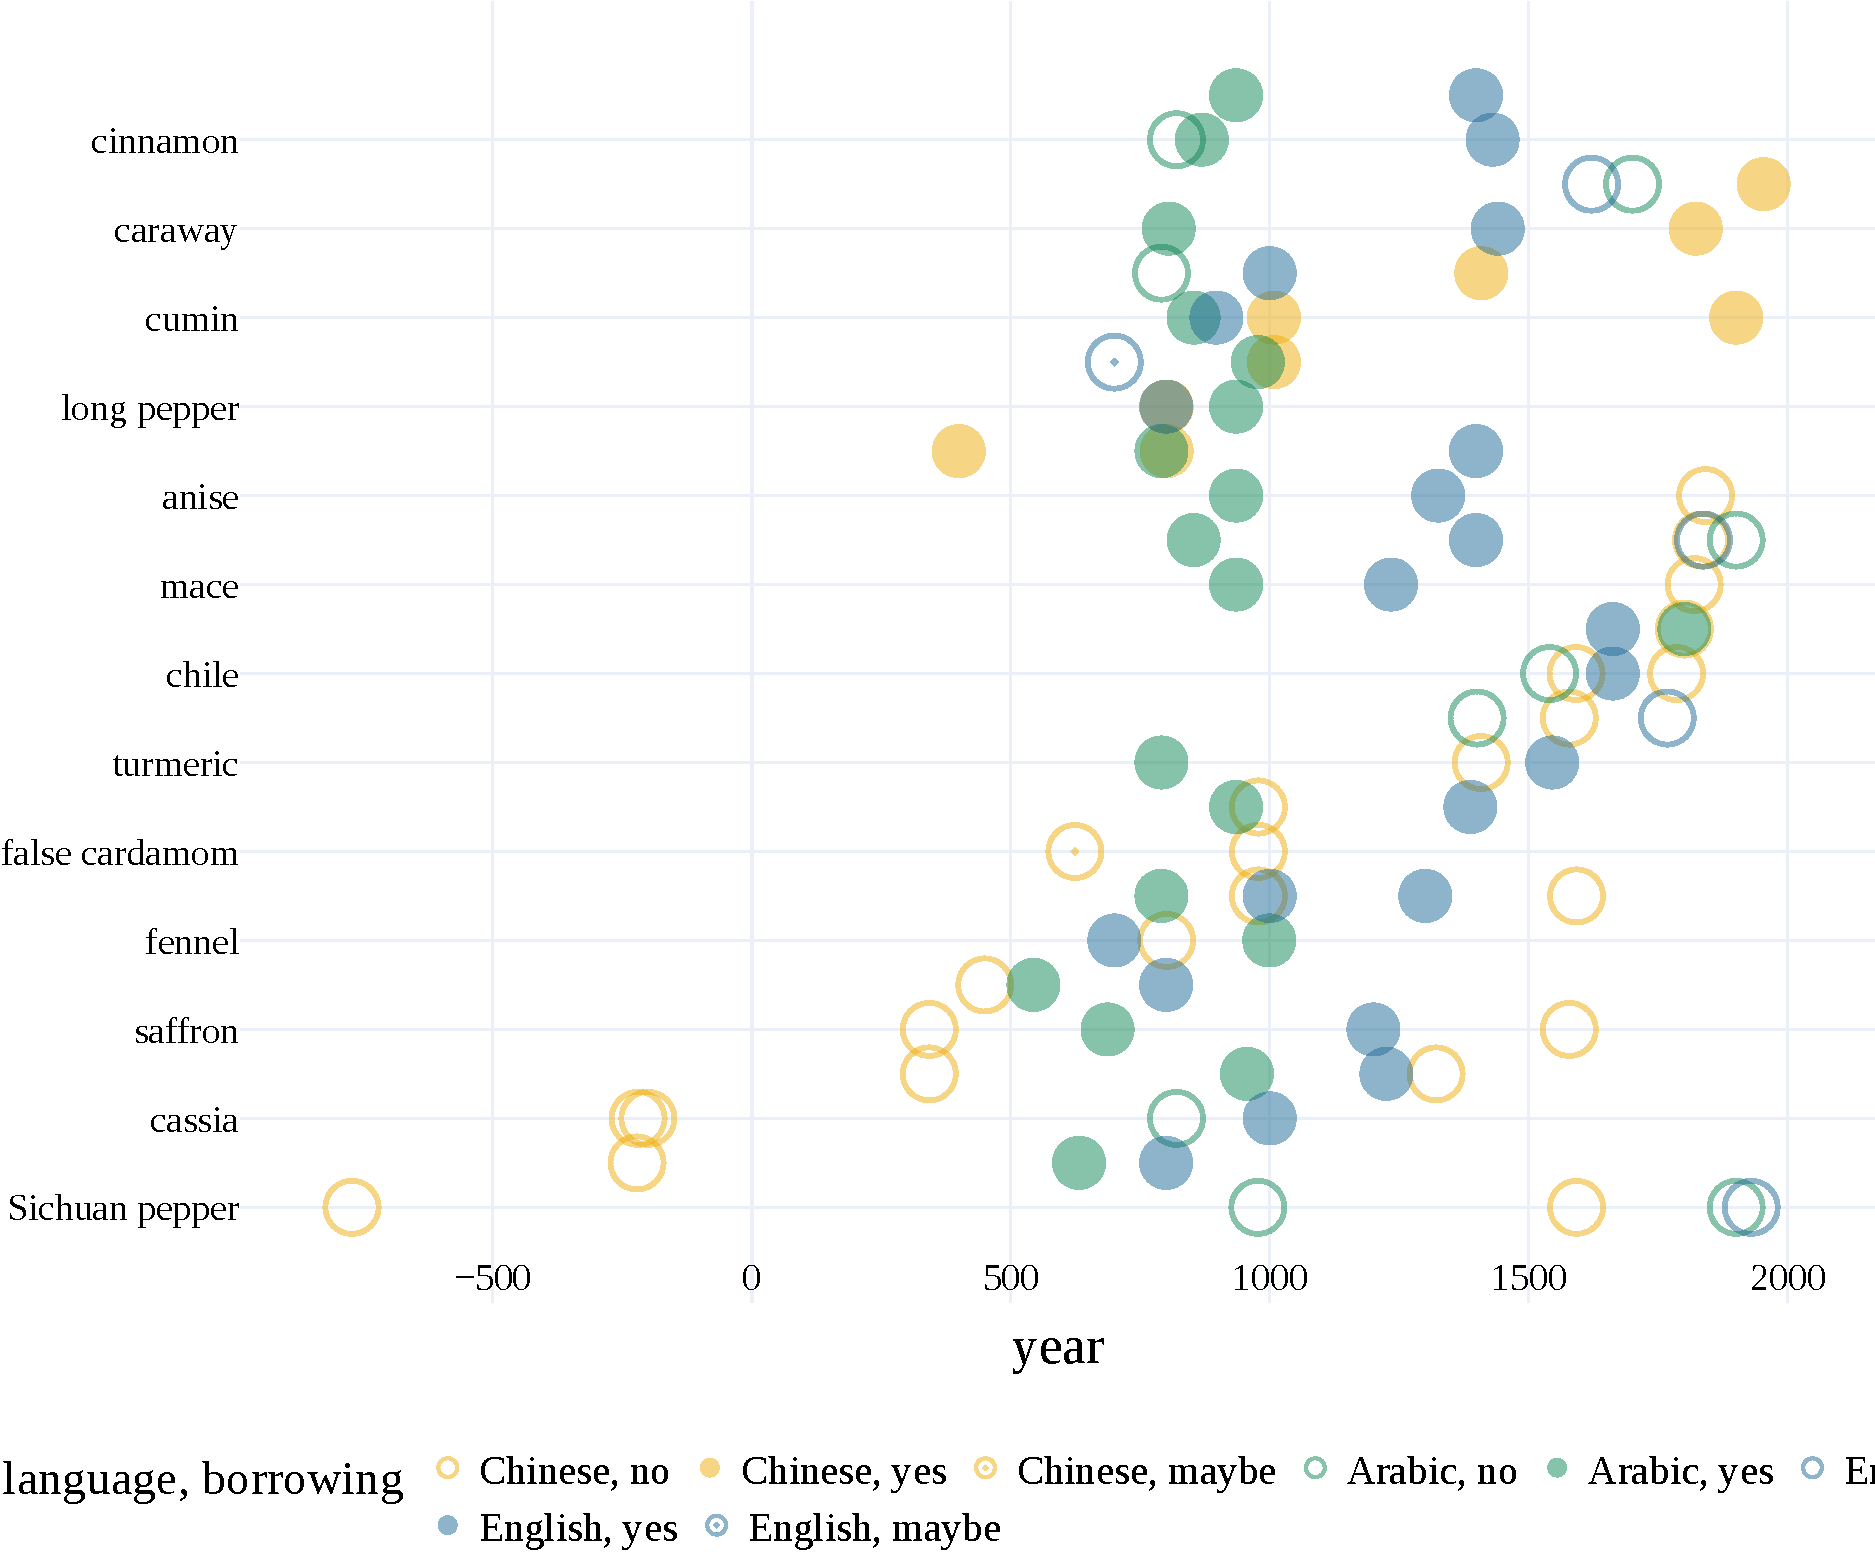
\includegraphics[width=\linewidth]{imgs/plots/borrowing.pdf}
  \caption{Borrowed spice terms across the three languages}
  \label{fig:borrowing}
\end{figure}

\begin{figure}[!ht]
  \centering
  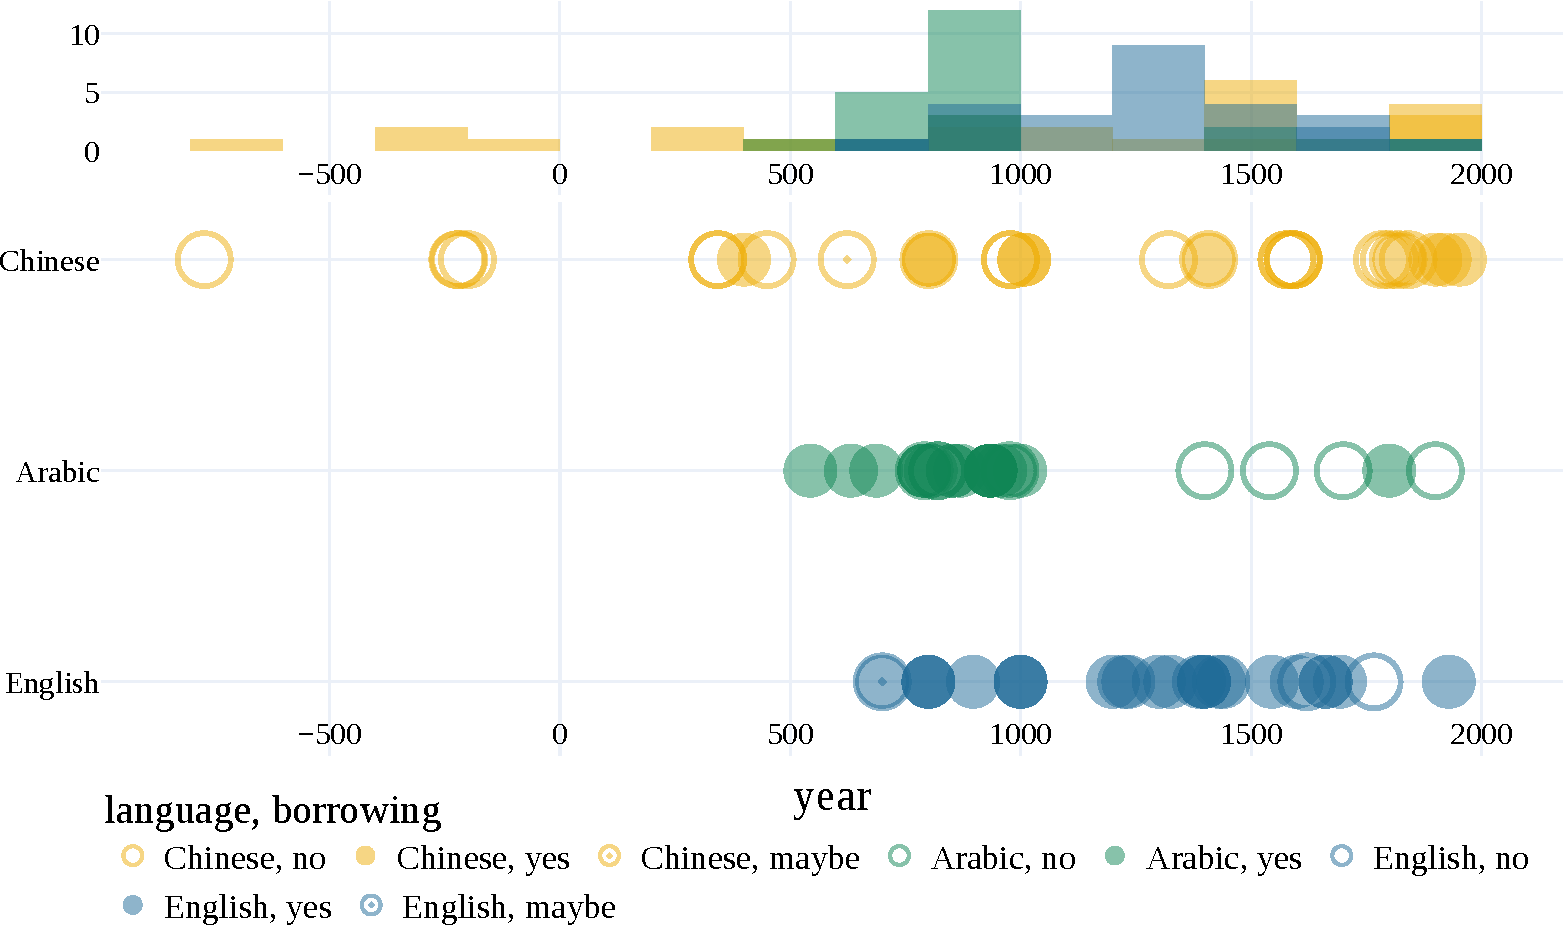
\includegraphics[width=\linewidth]{imgs/plots/borrowing_compact.pdf}
  \caption{}
  \label{fig:borrowing_compact}
\end{figure}

\subsection{Donor Languages}

\begin{figure}[!ht]
  \centering
  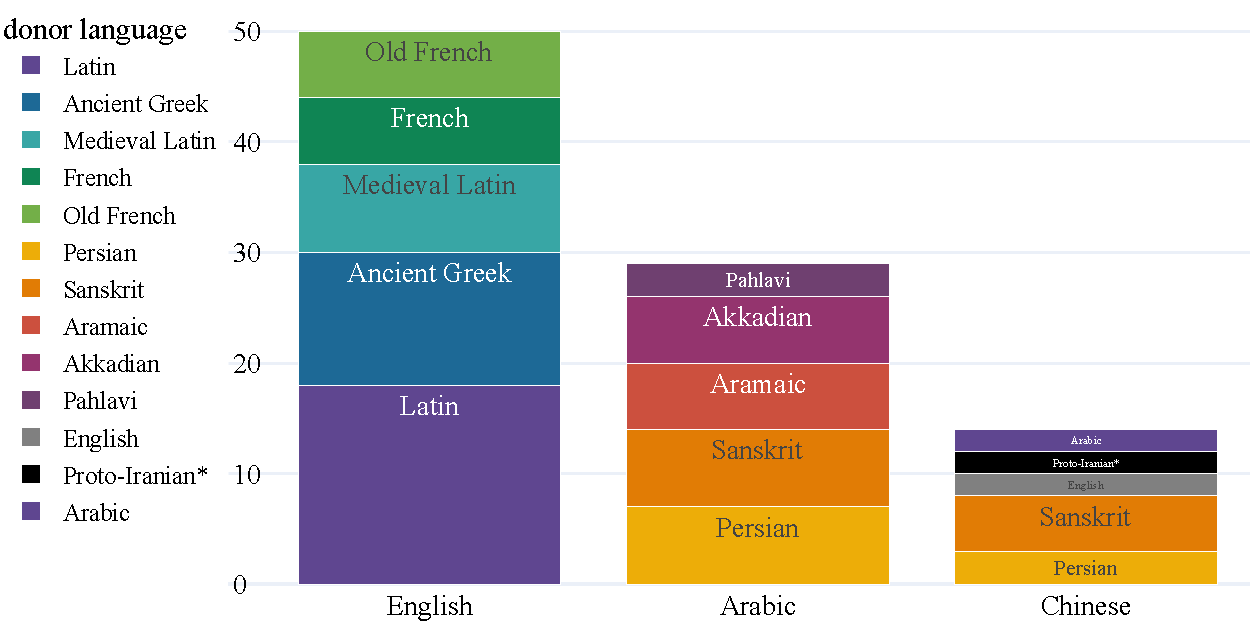
\includegraphics[width=\linewidth]{imgs/plots/donor_bar.pdf}
  \caption{}
  \label{fig:donor_bar}
\end{figure}




% mechanism


% The mechanisms of linguistic acculturation can be deducted from linguistic (and historical) analysis. 
% Is it borrowed or not, and if not, how speakers came up with the name?
% Spices and their spread are related to trade and cultural interaction 
% 	language contact

%     Linguistic acculturation “Response in a language to new items that become known through cultural contact. As the speakers of a language in contact with other cultures encounter new cultural items, they may:”
%     Borrow
%     Loan, calque (loan translate), learned loan…
%     Innovate
%     Compounding, blending, (internal resources)…
%     Shift
%     Narrowing, broadening, displacement…
%     Extend
%     metonymy (e.g.: octogon  bajiao; pentagon  The Pentagon)
%     metaphor
                                                
%                                                         (Campbell & Mixco, 2007)
%                               Borrowing
%                                                         Loanword			anise in English
%                                                         Loan translation		牙买加胡椒 [Jamaica pepper] in Mandarin; ‘allspice’
%                                                         Innovation
%                                                         Compounding		törökbors [Turkish-pepper] in Hungarian; ‘chilli’
%                                                         Folk-etymology		aniseed; safflower (morphological misinterpretation)
%                                                         Shift in meaning		
%                                                         Displacement			pimento in Spanish, replacing pebre ‘pepper’
%                                                         Extension
%                                                         Metonymy			bajiao [octagon] in Chinese; star anise
                                                        
                                                        
                                          


% Star anise is native to South China and Vietnam, fennel is native from Mediterranean to West Asia until the Himalayas. 
% Star anise has been used for around 3000 years (in and around the South, only later in the North), no longer found in the wild.
% The other plants I mentioned are all related to fennel, all are from the Apiaceae, the carrot/celery/parsley family (vt+ coriander 芫荽 and asafoetida 阿魏).
% They all look similar and are used similarly and named after each other in many languages.
% All these plants arrived from the west through Central Asia and the Silk Road.
% This is reflected in some of the names.
% What’s the connection between anise, star anise and fennel?
% Anethole – similar flavor profiles because of the same essential oil

% Is the name native or borrowed?
% The Chinese name is a native Chinese lexical “creation”
% English and Arabic used a non-native headword (anise, a loanword ultimately from Greek<Egyptian?), and a native distinguishing word (star) 


% These names are analyzable. 
% analysability of words is an idea from the philological movement Wörter und Sachen (words and things), which proposed the close study of etymology of words together with the artifacts/concepts.
% The more opaque a name is in terms of morphological analysis, the longer it is assumed to be present in the language.
% E.g.: York (monomorphemic) vs. New York (analysable)  provides a potential chronology
% Incorporated into historical linguistics ( + archeology)




% Just a quick question:
% I couldn't not notice that the character used for fennel and anise 茴 huí is made up of the radical for "grass" and 回 huí which is used for Islam and Muslims in Tang dynasty times. My question is: Could this be a construction that would refer to fennel (or anise) as "Muslim grass", "Muslim herb", since the plant came to China from the West originally (East Mediterranean, Middle East), and most likely through Muslim traders of Central Asia?
% Or this is not how Chinese characters work, and it is just my fantasy running wild and 回 huí is just a sound component...

% Thank you for the answer, I am working on the Tastes of Words article hastily now, I should be done very soon.



% Yes, good observation!  I suspected so too, but could not find direct supporting evidence yet.

% Good indirect evidences, other than your observation, are 
% >that 茴 is not found in Shuowenjiezi, which means that it is a later coinage and most likely borrowing; and in this case, 香 standing for herb in a compound and the first character will typically specify its origin (if borrowed), or plant, or sound
% >the earliest documented usage we can see now of this term is after Tang dynasty (supporting the borrowing hypothesis and consistent with the time of introduction of this herb to China)
% >The only document I found claims that it is derived from 蘾 from SWJZ characters due to phonological similarity. But this is an apparent 'backformation' speculation as 1) the phonology is distinctive enough (huai2 in Mandardin), and 2) it is a kind of watergrass in SWJZ, and definitely no fennel (and of course we do know now that China did not have fennel during SWJZ time)



% \section{What's in a name?}






% \section{Prototype Spices}

% \begin{itemize}
%     \item cardamom
%     \item pepper
% \end{itemize}


% cumin
% anise
% cinnamon
% saffron

